\documentclass{standalone}

\usepackage{tikz,pgf} %and any other packages or tikzlibraries your picture needs

\usepackage{pgfplots}
\usepackage[letterpaper,top=2cm,bottom=2cm,left=2cm,right=2cm,marginparwidth=1.75cm]{geometry}
\usepackage{mathtools} 
\usepackage{forest}
\usepackage{standalone}
\usepackage{pgfplots}
\usepackage{graphicx}
\usepackage{svg}
\usepackage{array}
\usepackage{pgfplots}
\usepackage{tikz}
\usepackage[utf8]{inputenc}
\usepackage[colorlinks=true, allcolors=blue]{hyperref}
\usetikzlibrary{positioning, arrows.meta, fit, shapes}
\begin{document}


 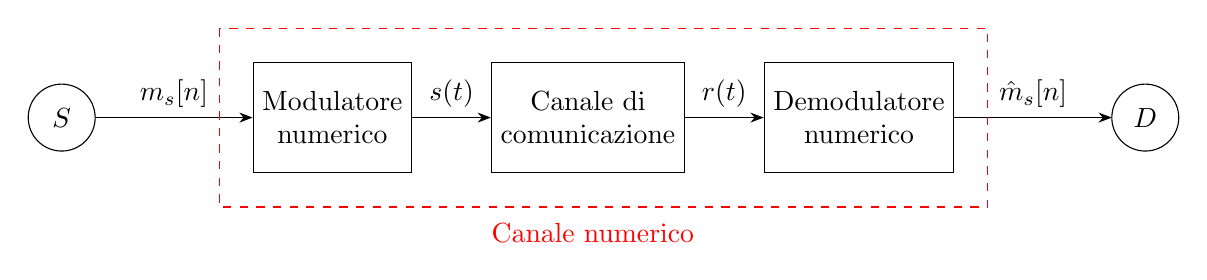
\begin{tikzpicture}[>=Stealth, block/.style={draw, rectangle}, scale=0.85]
            % Blocks
            \tikzstyle{block} = [rectangle, draw, text centered, minimum height=4em, align=center]

            \node[block] (mod) {Modulatore \\ numerico};
            \node[block, right=1cm of mod] (channel) {Canale di \\ comunicazione};
            \node[block, right=1cm of channel] (demod) {Demodulatore \\ numerico};

            % Nodes for connecting lines
            \coordinate[left=2cm of mod] (input);
            \coordinate[right=2cm of demod] (output);

            % Lines
            \draw[->] (input) -- node[above] {$m_s[n]$} (mod);
            \draw[->] (mod) -- node[above] {$s(t)$} (channel);
            \draw[->] (channel) -- node[above] {$r(t)$} (demod);
            \draw[->] (demod) -- node[above] {$\hat{m}_s[n]$} (output);

            % Dashed box
            \begin{scope}
                \draw[dashed, red] ($(mod.north west)+(-0.5,0.5)$) rectangle ($(demod.south east)+(0.5,-0.5)$);
            \end{scope}

            % Annotations
            \node[align=center, red, above right= -1cm and -6cm of demod.south east] (channel-label) {Canale numerico};

            % Circles
            \draw (input) ++(-0.5cm,0) circle (0.5cm) node {$S$};
            \draw (output) ++(0.5cm,0) circle (0.5cm) node {$D$};
        \end{tikzpicture}












\end{document}
